\chapter{Quantum Entanglements, Part 1}

These notes follow Leonard Susskind's opening lecture on quantum entanglement, with curation by LazyingArt LLC. The lecture begins in an unusual place. Instead of starting with the Schr\"odinger equation, it begins with a warning about intuition, then rebuilds the subject from the notions of information, configuration, update, and finally the elementary matrix algebra that will carry the quantum theory in the next lecture.

\section{Why Quantum Mechanics Feels Unnatural}

Susskind opens with the sermon he says he almost always gives. Our physical intuitions were not trained on electrons, uncertainty, or motion near the speed of light. They were trained on rocks, arrows, falling bodies, prey, predators, and the moderate scales of ordinary experience. A lion chasing an antelope is already solving a sophisticated kinematical problem, but it is solving the problem that evolution prepared it to solve. In that sense classical mechanics feels natural because our brains were built under conditions in which something like classical mechanics is useful every day.

Modern physics begins precisely where such inherited intuition fails. Relativity asks us to reason in regimes where ordinary velocity addition breaks down. Quantum mechanics asks us to reason about objects for which even the basic picture of a particle as a thing with a trajectory becomes unreliable. There is no reason to expect an untutored visual imagination to be at home there. The appropriate response is not despair, but rewiring: one learns new abstractions until they become the new intuition.

That is the point of departure for the whole course. We are not going to proceed as a conventional quantum mechanics course would proceed, with waves and the Schr\"odinger equation at center stage from the beginning. The emphasis here is different. We are after the logic of quantum mechanics and, more specifically, the logic of quantum information. The first serious object, therefore, is not the wave function but the bit.

\section{Classical Bits and the Counting of States}

Physics, in this telling, is information. To say something about a physical system is to supply information about it, often in the form of numbers and sometimes in the form of simple yes-or-no alternatives. A two-valued question is the prototype.

\begin{definition}
A bit is a question about a system with only two possible answers.
\end{definition}

Heads or tails, up or down, yes or no: logically these are the same structure. Before the quantum version is introduced, Susskind deliberately slows down and discusses the classical version. The two classical values may be labeled in any convenient way, but the lecture settles on \(0\) and \(1\). One may think of these as heads and tails, or as any other two-valued distinction.

He then introduces Dirac notation earlier than one might expect. At this stage the notation looks redundant, and he says so. But it is installed now because it will matter later.

\begin{equation}
|0\rangle,\qquad |1\rangle
\end{equation}

These are not yet quantum superpositions. They are simply two classical configurations written in a notation that will survive the transition to quantum mechanics. The bracketed object is called a ket.

For several bits, we simply write a string. A configuration of many bits is therefore written schematically as

\begin{equation}
|001011\cdots\rangle.
\end{equation}

The next question comes naturally: how many distinct configurations are available? One bit has two states. Two bits have four. In general, each new bit doubles the number of possibilities. Thus an \(n\)-bit system has

\begin{equation}
N_s = 2^n
\end{equation}

possible classical configurations, where \(N_s\) denotes the number of states. Inverting the relation gives

\begin{equation}
n = \log_2 N_s.
\end{equation}

This is the first quantitative measure of information in the lecture. If the number of states is not itself a power of two, the logarithm still makes sense. A die has six states, so the amount of information it can carry is \(\log_2 6\), which is not an integer. The point is not that every system comes packaged as a perfect collection of binary alternatives, but that the amount of information is measured by the base-two logarithm of the number of available states.

\section{How Ordinary Physics Becomes a Bit String}

At this point the lecture could easily remain a discussion of coins and toy logical systems. Instead Susskind broadens the meaning of a bit. The important claim is that ordinary physical information can usually be encoded, at least approximately, by a long enough string of binary data.

Take a number such as the temperature of a room. If we care only about finite accuracy, we may truncate the description and write the resulting number in base two. Then the numerical value is represented by a sequence of zeros and ones. The same is true of any measured quantity when finite precision is enough for the purpose at hand.

The same idea extends to fields. A field is something that varies from place to place. To encode it in bits we discretize space, cutting the room into many small cells and assigning an ordered list to those cells. We then record the value of the field in each cell, again only to finite precision and again in binary notation. What comes out is one long binary description of the field configuration.

The lecture pushes the same idea one step further with a lattice occupancy example. Suppose each cell is either occupied by a particle or empty. Then each cell carries one bit:

\begin{equation}
\text{occupied} \longleftrightarrow 1,
\qquad
\text{empty} \longleftrightarrow 0.
\end{equation}

A whole particle configuration is then nothing more than a string of zeros and ones. In this sense the positions of particles, the values of fields, and ordinary macroscopic quantities can all be encoded by bit strings.

There is, of course, a caveat. If we insist on exact classical real numbers, then irrational values require infinitely many bits, and even rational values may require repeating descriptions. The lecture does not hide that. But its operational point is simpler: digital computation works because physically useful descriptions can be approximated by finite bit strings, and made more accurate by using more bits and finer lattices.

\section{Configurations, Update Rules, and State Space}

Once the lecture has explained how to encode a system, it changes register. A physical theory is not merely a catalogue of allowed configurations. It must also tell us how one configuration becomes another.

\begin{definition}
A configuration is the state of a system at a given instant of time.
\end{definition}

So far we have mostly discussed configuration. Now we add dynamics. Space may be discretized into cells; time may also be discretized, at least as a convenience. Then the motion of the system is represented by a rule that updates one configuration into the next.

This gives a very spare summary of classical physics in the lecture's language: a system consists of a collection of possible states, together with a rule of updating that takes the state at one instant to the state at a slightly later instant.

To make this visible, Susskind introduces the abstract state space. One should not confuse this with ordinary space. Its points are not positions in the room. They are configurations of the whole system. For a one-bit system the state space has only two points. One possible law is the trivial one: heads stays heads and tails stays tails. Another law is the flip-flop: heads goes to tails and tails goes to heads.

The same idea extends to two bits. A two-bit system has four states, and different laws correspond to different arrow patterns among those four configurations. Some laws form closed loops. Some describe two separate flip-flops running in parallel. The lecture keeps the discussion deliberately elementary. The goal is not to classify all possible dynamical systems, but to make it clear what a law of motion looks like when represented as updating in logical state space.

\section{Reversibility, Information Loss, and Unitarity}

The next move is the conceptual center of the lecture. After showing several perfectly acceptable update rules, Susskind draws another one that is logically easy to imagine but physically defective. Two different initial states flow into the same later state. Going forward is still possible, but going backward is no longer unique. Information has been lost.

\begin{figure}[h]
\centering

\includegraphics[width=0.72\textwidth]{lecture_01_figure_02.png}
\caption{Board sketch from the discussion of reversible and irreversible update laws, with the handwritten word \emph{unitarity}.}
\end{figure}

\begin{figure}[h]
\centering
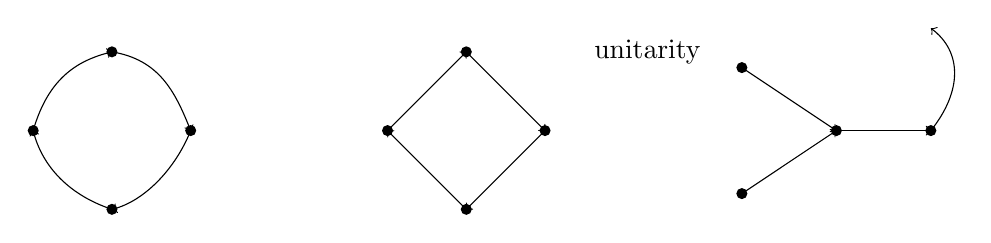
\begin{tikzpicture}[scale=1.0]
\fill (0,1) circle (2pt);
\fill (1,2) circle (2pt);
\fill (2,1) circle (2pt);
\fill (1,0) circle (2pt);
\draw[->] (0,1) .. controls (0.2,1.7) and (0.6,1.9) .. (1,2);
\draw[->] (1,2) .. controls (1.6,1.9) and (1.8,1.5) .. (2,1);
\draw[->] (2,1) .. controls (1.8,0.5) and (1.4,0.1) .. (1,0);
\draw[->] (1,0) .. controls (0.4,0.2) and (0.1,0.6) .. (0,1);

\fill (4.5,1) circle (2pt);
\fill (5.5,2) circle (2pt);
\fill (6.5,1) circle (2pt);
\fill (5.5,0) circle (2pt);
\draw[->] (4.5,1) -- (5.5,2);
\draw[->] (5.5,2) -- (6.5,1);
\draw[->] (6.5,1) -- (5.5,0);
\draw[->] (5.5,0) -- (4.5,1);
\node at (7.8,2) {unitarity};

\fill (9.0,1.8) circle (2pt);
\fill (9.0,0.2) circle (2pt);
\fill (10.2,1.0) circle (2pt);
\fill (11.4,1.0) circle (2pt);
\draw[->] (9.0,1.8) -- (10.2,1.0);
\draw[->] (9.0,0.2) -- (10.2,1.0);
\draw[->] (10.2,1.0) -- (11.4,1.0);
\draw[->] (11.4,1.0) .. controls (11.8,1.5) and (11.8,2.0) .. (11.4,2.3);
\end{tikzpicture}
\caption{A clean schematic reconstruction of the board logic: reversible loops on the left, and an information-losing update pattern on the right.}
\end{figure}

The acceptable diagrams have a common feature. Each state has one definite next state, and also one definite previous state. In Susskind's language, there is a unique future and a unique past. This is the sense in which the law is reversible.

\subsection{Question \& Answer}

\paragraph{Question.} Why is the apparently sensible merging update rule forbidden? After all, it tells us exactly where the system goes next.

\paragraph{Answer.} It is forbidden because it destroys the distinction between different pasts. If two different states both flow into the same later state, then the present no longer contains enough information to reconstruct the past. The law still gives a future, but it does not give a unique past. That is what Susskind means by loss of information. At the fundamental level, where we are keeping track of every degree of freedom and not coarse-graining, classical physics does not allow such loss.

This does \emph{not} mean that every reversible law is invariant under naive time reversal. A cyclic diagram still has an orientation: it runs one way under forward evolution. The point is subtler. Given the forward law, one can construct a reverse law that takes us back uniquely. The lecture therefore distinguishes reversibility from exact time-reversal symmetry.

The same section of the lecture also addresses a natural objection. In thermodynamics it often looks as if information is lost: gas released from one corner of a room spreads everywhere, and many different initial macroscopic arrangements seem to end in the same final macroscopic state. Susskind's reply is that this is usually coarse-grained loss. If we followed every molecule with enough precision, then in principle the microscopic information would still be there. What is lost in practice is not the information itself, but our ability to keep track of it.

Finally he names the quantum analog of this uniqueness property. In quantum mechanics, he says, the corresponding principle is called \emph{unitarity}. The lecture does not yet formalize that statement in matrix language. For now it serves as a preview: quantum evolution, too, will be required to carry enough structure that past and future are uniquely related.

\section{Vectors, Rows, Columns, and Inner Products}

After the break, the lecture pivots sharply but not arbitrarily. If the laws of physics are to be encoded as update rules, then we need a clean algebraic language for those updates. That language begins with vectors.

A vector is introduced here in the least metaphysical way possible: it is simply a finite sequence of numbers. At this stage the entries are taken to be real numbers. Susskind explicitly postpones the passage to complex numbers and the dagger notation.

A four-component vector may be written as a row,

\begin{equation}
A=(A_1,A_2,A_3,A_4),
\end{equation}

or as a column,

\begin{equation}
A=
\begin{pmatrix}
A_1\\
A_2\\
A_3\\
A_4
\end{pmatrix}.
\end{equation}

The two notations contain the same data. They are useful in different operations.

\begin{figure}[h]
\centering

\includegraphics[width=0.45\textwidth]{lecture_01_figure_03.png}
\caption{The board at the moment the lecture turns from state diagrams to column-vector notation.}
\end{figure}

Next comes the inner product. Let

\begin{equation}
B=(B_1,B_2,B_3,B_4)
\end{equation}

be a row vector, and let \(A\) be the column vector above. Their product is defined by multiplying corresponding entries and summing:

\begin{equation}
BA = B_1A_1+B_2A_2+B_3A_3+B_4A_4.
\end{equation}

The result is a number, not a new vector. In ordinary Euclidean language this would be the dot product. Here Susskind emphasizes the more abstract name \emph{inner product}. The important operational point is that rows multiply columns to produce scalars.

\section{Matrices as Update Operators}

A matrix is now introduced as a machine that acts on a vector and produces another vector. Again the lecture avoids formalism for its own sake. The matrix is valuable because it packages useful update rules.

Write a \(4\times4\) matrix as

\begin{equation}
M=
\begin{pmatrix}
M_{11} & M_{12} & M_{13} & M_{14}\\
M_{21} & M_{22} & M_{23} & M_{24}\\
M_{31} & M_{32} & M_{33} & M_{34}\\
M_{41} & M_{42} & M_{43} & M_{44}
\end{pmatrix}.
\end{equation}

It acts on the column vector \(A\) by taking each row of the matrix and forming its inner product with the column. In compact notation,

\begin{equation}
(MA)_i=\sum_j M_{ij}A_j,
\end{equation}

and the first two components are
\begin{align}
(MA)_1 &= M_{11}A_1+M_{12}A_2+M_{13}A_3+M_{14}A_4,\\
(MA)_2 &= M_{21}A_1+M_{22}A_2+M_{23}A_3+M_{24}A_4.
\end{align}

\begin{figure}[h]
\centering

\includegraphics[width=0.82\textwidth]{lecture_01_figure_04.png}
\caption{Board layout for the discussion of a matrix acting on a column vector.}
\end{figure}

This is already enough to represent classical evolution. Susskind begins with a cycle of states, briefly tries to draw it for five states, then sensibly retreats to four so that the arithmetic can fit on the board. The key idea is to encode the classical states by one-hot vectors:
\begin{equation}
e_1=
\begin{pmatrix}
1\\0\\0\\0
\end{pmatrix},
\qquad
e_2=
\begin{pmatrix}
0\\1\\0\\0
\end{pmatrix},
\qquad
e_3=
\begin{pmatrix}
0\\0\\1\\0
\end{pmatrix},
\qquad
e_4=
\begin{pmatrix}
0\\0\\0\\1
\end{pmatrix}.
\end{equation}

A cyclic update \(1\to2\to3\to4\to1\) can then be represented by the permutation matrix
\begin{equation}
P=
\begin{pmatrix}
0&0&0&1\\
1&0&0&0\\
0&1&0&0\\
0&0&1&0
\end{pmatrix}.
\end{equation}

This convention is chosen cleanly here; on the board Susskind corrects the direction live, so only the cyclic logic is stable, not the literal orientation of the first draft. With this choice we have
\begin{equation}
Pe_1=e_2,\qquad
Pe_2=e_3,\qquad
Pe_3=e_4,\qquad
Pe_4=e_1.
\end{equation}

The same matrix acts on a general column by shifting entries cyclically:
\begin{equation}
P
\begin{pmatrix}
A\\B\\C\\D
\end{pmatrix}
=
\begin{pmatrix}
D\\A\\B\\C
\end{pmatrix}.
\end{equation}

That is the worked example the lecture wants us to see: a law of motion becomes a matrix.

Now suppose we update twice. If one update is
\begin{equation}
V'=MV,
\end{equation}
then a second update gives
\begin{equation}
V''=MV'=M^2V.
\end{equation}
So matrix multiplication composes time evolution.

\begin{figure}[h]
\centering

\includegraphics[width=0.72\textwidth]{lecture_01_figure_05.png}
\caption{Board layout for multiplying a \(2\times2\) matrix by the columns of another matrix.}
\end{figure}

To keep the arithmetic manageable, Susskind switches to \(2\times2\) matrices. Let
\begin{equation}
M=
\begin{pmatrix}
M_{11} & M_{12}\\
M_{21} & M_{22}
\end{pmatrix},
\qquad
N=
\begin{pmatrix}
N_{11} & N_{12}\\
N_{21} & N_{22}
\end{pmatrix}.
\end{equation}
Then the product \(C=MN\) is another matrix, whose entries are found by multiplying rows of \(M\) by columns of \(N\). The first entry is
\begin{equation}
C_{11}=M_{11}N_{11}+M_{12}N_{21}.
\end{equation}
The next one is
\begin{equation}
C_{12}=M_{11}N_{12}+M_{12}N_{22}.
\end{equation}
In clean general notation,
\begin{equation}
C_{ij}=\sum_k M_{ik}N_{kj}.
\end{equation}

This is exactly the interpretation suggested by the board layout: the right-hand matrix can be read as a collection of column vectors, each of which is acted on by the left-hand matrix.

The lecture ends by adding the final pattern. A row vector can also multiply a matrix. If
\begin{equation}
B=(B_1,B_2,B_3,B_4),
\end{equation}
then \(BM\) is a row vector whose \(j\)-th entry is obtained by multiplying the row \(B\) by the \(j\)-th column of \(M\):
\begin{equation}
(BM)_j=\sum_i B_iM_{ij}.
\end{equation}

Rows times columns give numbers, matrices times columns give columns, rows times matrices give rows, and matrices times matrices give matrices. Susskind's final pedagogical point is unmistakable: if we are comfortable with these operations, then we already possess the elementary algebra that quantum mechanics will soon require.

A question at the end of the lecture pushes one more step. What restriction does reversibility place on a matrix? The answer is that the update matrix should have an inverse. In other words, reversible evolution is represented by a matrix that can be undone. The lecture does not yet develop that criterion in detail, but it is the right algebraic echo of the earlier discussion of unique past and unique future.

\section{Summary}

The first lecture does not yet enter quantum mechanics proper. Instead it clears the ground. We are told why ordinary intuition is an unreliable guide, why physics may be recast as information, how classical configurations are encoded by bits, why counting states leads naturally to logarithmic measures of information, and why a physical theory must specify both a space of configurations and an update rule.

Only after that groundwork does the algebra appear. Vectors, inner products, matrices, and matrix multiplication are not an isolated review session. They are the language in which update laws will shortly be expressed. The lecture therefore ends exactly where it should end: with classical bits encoded in linear algebra, and with qubits waiting just beyond the door.